%15 min preso!
\documentclass[xcolor=table,aspectratio=169]{beamer}
\usepackage{beamerthemesplit}
\usepackage{wrapfig}
\usetheme{SPbGU}
\usepackage{pdfpages}
\usepackage{amsmath}
\usepackage{cmap}
\usepackage[T2A]{fontenc}
\usepackage[utf8]{inputenc}
\usepackage[english]{babel}
\usepackage{indentfirst}
\usepackage{amsmath}
\usepackage{tikz}
\usepackage{multirow}
\usepackage[noend]{algpseudocode}
\usepackage{algorithm}
\usepackage{algorithmicx}
\usepackage{fancyvrb}
\usepackage{hyperref} 
\usetikzlibrary{calc}
\usetikzlibrary{shapes,arrows}
\usetikzlibrary{arrows,automata}
\usetikzlibrary{positioning}

\usepackage{tabularx}
\newcolumntype{Y}{>{\raggedleft\arraybackslash}X}

\renewcommand{\thealgorithm}{}

\newtheorem{mytheorem}{Theorem}
\renewcommand{\thealgorithm}{}

\newcommand{\tikzmark}[1]{\tikz[overlay,remember picture] \node (#1) {};}
\def\Put(#1,#2)#3{\leavevmode\makebox(0,0){\put(#1,#2){#3}}}

\newcommand{\ltz}{$< 1$}


\tikzset{
    state/.style={
           rectangle,
           rounded corners,
           draw=black, very thick,
           minimum height=2em,
           inner sep=2pt,
           text centered,
           },
}

\beamertemplatenavigationsymbolsempty

\title[Graph analysis \& Graph DB]{Graph Analysis and Graph Databases}
\institute[PL\&T@SPbSU]{
Saint Petersburg State University
}

% То, что в квадратных скобках, отображается в левом нижнем углу.
\author[Semyon Grigorev]{Semyon Grigorev}

\date{April 16, 2022}

\begin{document}
{
\begin{frame}[fragile]
  \begin{table}
  \centering
  
\includegraphics[height=1.5cm]{pictures/SPbGU_Logo.png}
  %\begin{tabularx}{\linewidth}{XcX}
    %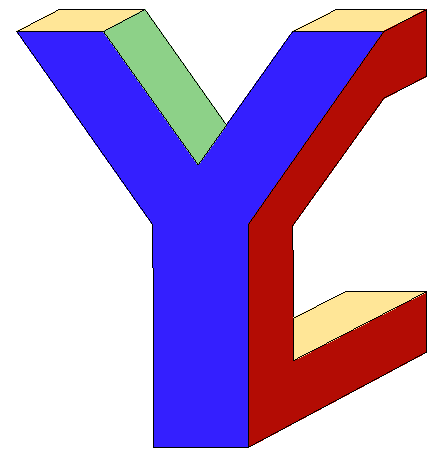
\includegraphics[height=1.5cm]{pictures/YC_logo.pdf} \hfill
    %& \begin{minipage}[t]{0.3\textwidth}\center \vspace{-1cm}  %Huawei-SPbSU Open Day 2021
    %  \end{minipage}
    %& \hfill 
\includegraphics[height=1.5cm]{pictures/SPbGU_Logo.png}
  %\end{tabularx}
  \end{table}
  \titlepage
\end{frame}
}

\begin{frame}[fragile]
  \frametitle{Group Info}  
  \begin{itemize}      
      \item Lead: Semyon Grigorev
      \begin{itemize}
        \item PhD (2016), Associate professor (2016, SPbSU)
        \item dblp: \href{https://dblp.org/pid/181/9903.html}{https://dblp.org/pid/181/9903.html}
        \item \href{s.v.grigoriev@spbu.ru}{s.v.grigoriev@spbu.ru}
      \end{itemize}
      \item PhD students: 2
      \item Master students: 2
      \item Bachelor students: 4
      \pause
      \item Research areas
      \begin{itemize}
        \item High-performance graph analysis        
        \item Formal languages constrained path querying  
        \item Graph databases and graph query languages      
      \end{itemize}
    \end{itemize}
\end{frame}


\begin{frame}[fragile]
  \frametitle{High-Performance Graph Analysis}
  \begin{itemize}
    \item Linear algebra based algorithms for graph analysis
    \begin{itemize}
      \item Parallel algorithms on CPU and GPGPU
      \item Sparse linear algebra
      \item GraphBLAS API
    \end{itemize} 
    \pause
    \item Research directions
    \begin{itemize}
      \item GraphBLAS-based algorithms design, implementation and evaluation      
      \item Integration of algorithms to graph databases
      \item Portable multi-GPGPU implementation of GraphBALS-like API            
    \end{itemize}
    \pause
    \item Collaboration
    \begin{itemize}
      \item GraphBLAS community
      \item LDBC community
    \end{itemize}

  \end{itemize}
\end{frame}


\begin{frame}[fragile]
  \frametitle{High-Performance Graph Analysis: Results}
    \begin{itemize}
      \item Tools
      \begin{itemize}
        \item \href{https://github.com/JetBrains-Research/spla}{Spla: sparse linear algebra framework for multi-GPU computations based on OpenCL}
        \item \href{https://github.com/JetBrains-Research/spbla}{SPbLA: library of GPGPU-powered sparse boolean linear algebra operations}    
        \item \href{https://github.com/JetBrains-Research/ldbc_graphalytics}{LDBC Graphalytics extension for evaluation of formal language constrained path querying}    
      \end{itemize}
      \item Papers 
      \begin{itemize}
        \item SPbLA: The Library of GPGPU-Powered Sparse Boolean Linear Algebra Operations (GrAPL@IPDPS)
        \item Evaluation of the context-free path querying algorithm based on matrix multiplication (GRADES-NDA@SIGMOD)
      \end{itemize} 
    \end{itemize}
\end{frame}

\begin{frame}[fragile]
  \frametitle{Formal Language Constrained Path Querying (FLPQ)}
  \begin{itemize}
    \item Formal languages as path constraints 
    \begin{itemize}
      \item Regular path querying (RPQ)
      \item Context-free path querying (CFPQ)
    \end{itemize} 
    \begin{itemize}
    \item Applications 
    \begin{itemize}
      \item Graph analysis
      \item Interprocedural static code analysis
      \item Graph database querying
    \end{itemize}
  \end{itemize}
    \pause
    \item Research directions
    \begin{itemize}
      \item New algorithms development
      \item Complexity analysis
      \item High performance algorithms implementation and evaluation 
    \end{itemize}
    \pause
    \item Collaboration
    \begin{itemize}      
      \item LDBC community
      \item RedisGraph team
      \item Neo4j team
    \end{itemize}
  \end{itemize}
\end{frame}


\begin{frame}[fragile]
  \frametitle{FLPQ: Results}
    \begin{itemize}
      \item Tools
      \begin{itemize}
        \item \href{https://github.com/JetBrains-Research/GLL4Graph}{GLL4Graph: CFPQ for Neo4j}
        \item \href{https://github.com/YaccConstructor/RedisGraph}{CFPQ for RedisGraph}
        \item \href{https://github.com/JetBrains-Research/CFPQ_PyAlgo}{CFPQ\_PyAlgo: set of GrpapBLAS-based FLPQ algorithms}
      \end{itemize}
      \item Papers (> 10)
      \begin{itemize}
        \item Multiple-Source Context-Free Path Querying in Terms of Linear Algebra (EDBT, Core A)
        \item Context-free path querying by matrix multiplication (GRADES-NDA@SIGMOD)
        \item Parser combinators for context-free path querying (Scala@ICFP)
      \end{itemize} 
    \end{itemize}
\end{frame}


\end{document}
